\documentclass[aspectratio=169]{beamer}
\mode<presentation>

\usepackage{adjustbox}
\usepackage{array}
\usepackage{calc}
\usepackage{fancyvrb}
\usepackage{listings}
\usepackage{relsize}
\usepackage{graphicx}
\usepackage[most]{tcolorbox}
\usepackage[overlay,absolute]{textpos}
\usepackage{xcolor}

\graphicspath{{../images}}

\usepackage{fontspec}
\setsansfont{Helvetica Neue Light}[
    BoldFont={Helvetica Neue Bold},
    BoldItalicFont={Helvetica Neue Bold Italic},
    ItalicFont={Helvetica Neue Light Italic}
]
\setmonofont{Iosevka Term}
\newfontface\helvreg{Helvetica Neue}

\definecolor{grayish}{gray}{0.8}

\title{Concatenative programming\\and stack-based languages}
\author{Douglas Creager}
\institute{Walland Heavy Research}
\date{Strange Loop\\\textsmaller[1]{September 21–22, 2023 – St. Louis}}

\setbeamercolor{title}{fg=black}
\setbeamerfont{title}{series=\bfseries,size=\larger[1]}
\setbeamerfont{subtitle}{series=\mdseries,size=\smaller[2]}
\setbeamerfont{author}{size=\smaller[1]}
\setbeamerfont{institute}{size=\smaller[2]}
\setbeamertemplate{navigation symbols}{}
\setbeamercolor{frametitle}{fg=black}
\setbeamerfont{frametitle}{series=\bfseries}

% Picture credits

\makeatletter
\def\picturecredits{}
\newcommand{\picturecredit}[4]{
    \protected@xappto\picturecredits{
        \textsmaller[3]{Slide \theframenumber} &
        \textsmaller[2]{#1, “#2”} \vspace*{-0.4em} \newline
        \textsmaller[3]{#3, \url{#4}} \\
    }
}
\makeatother

\newlength{\titlewidth}
\newcommand{\flattitle}[3]{
    \settowidth{\titlewidth}{\textbf{\LARGE #3}}
    \begin{textblock*}{\titlewidth}(#1,#2)
        \textbf{\LARGE #3}
    \end{textblock*}
}
\newcommand{\shadowedtitle}[3]{
    \settowidth{\titlewidth}{\textbf{\LARGE #3}}
    \addtolength{\titlewidth}{0.5mm}
    \begin{textblock*}{\titlewidth}(#1+0.4mm,#2+0.4mm)
        \textbf{\LARGE #3}
    \end{textblock*}
    \begin{textblock*}{\titlewidth}(#1,#2)
        \textbf{\textcolor{white}{\LARGE #3}}
    \end{textblock*}
}

%%%%%%%%%%%%%%%%%%%%%%%%%%%%%%%%%%%%%%%%%%%%%%%%%%%%%%%%%%%%%%%%%%%%%%%%%%%%%%%%
% Program source

\lstset{
  basicstyle=\small\ttfamily,%
  columns=fullflexible,
  keepspaces=true,
  escapechar=?,
  extendedchars=true}

%%%%%%%%%%%%%%%%%%%%%%%%%%%%%%%%%%%%%%%%%%%%%%%%%%%%%%%%%%%%%%%%%%%%%%%%%%%%%%%%
% Simple stack language

\newdimen\origiwspc
\origiwspc=\fontdimen2\font

\newcommand<>{\stackex}[2]{%
    \begin{onlyenv}#3
    \begin{tabular}[c]{
        @{\extracolsep{1em}}
        >{\rule[-0.6\baselineskip]{0pt}{1.8\baselineskip}\raggedleft\arraybackslash\fontdimen2\font=1ex}p{0.3\textwidth}<{\fontdimen2\font=\origiwspc}
        |
        >{\strut\raggedright\arraybackslash\leavevmode\color{blue}\ttfamily}p{0.6\textwidth}
    }
        \cline{1-1}
        #1 & #2 \\
        \cline{1-1}
    \end{tabular}
    \end{onlyenv}%
    \ignorespaces
}

\newcommand{\sym}[1]{\textcolor{blue}{\texttt{#1}}}

\newcommand{\stacksplit}[2][]{%
    \tcbox[
        standard jigsaw,
        nobeforeafter,
        size=fbox,
        boxrule=0pt,
        sharp corners=all,
        #1
    ]{\sym{\strut#2}}%
    \ignorespaces
}

%%%%%%%%%%%%%%%%%%%%%%%%%%%%%%%%%%%%%%%%%%%%%%%%%%%%%%%%%%%%%%%%%%%%%%%%%%%%%%%%

\begin{document}

\begin{frame}
    \titlepage
\end{frame}

%%%%%%%%%%%%%%%%%%%%%%%%%%%%%%%%%%%%%%%%%%%%%%%%%%%%%%%%%%%%%%%%%%%%%%%%%%%%%%%%
% Initial stack language examples

\begin{frame}
    \begin{textblock*}{160mm}(0mm,0mm)
        \picturecredit{Marco Verch}{Stack of pancakes with berries on a plate}{CC-BY-2.0}{https://flic.kr/p/2jYUh8M}
        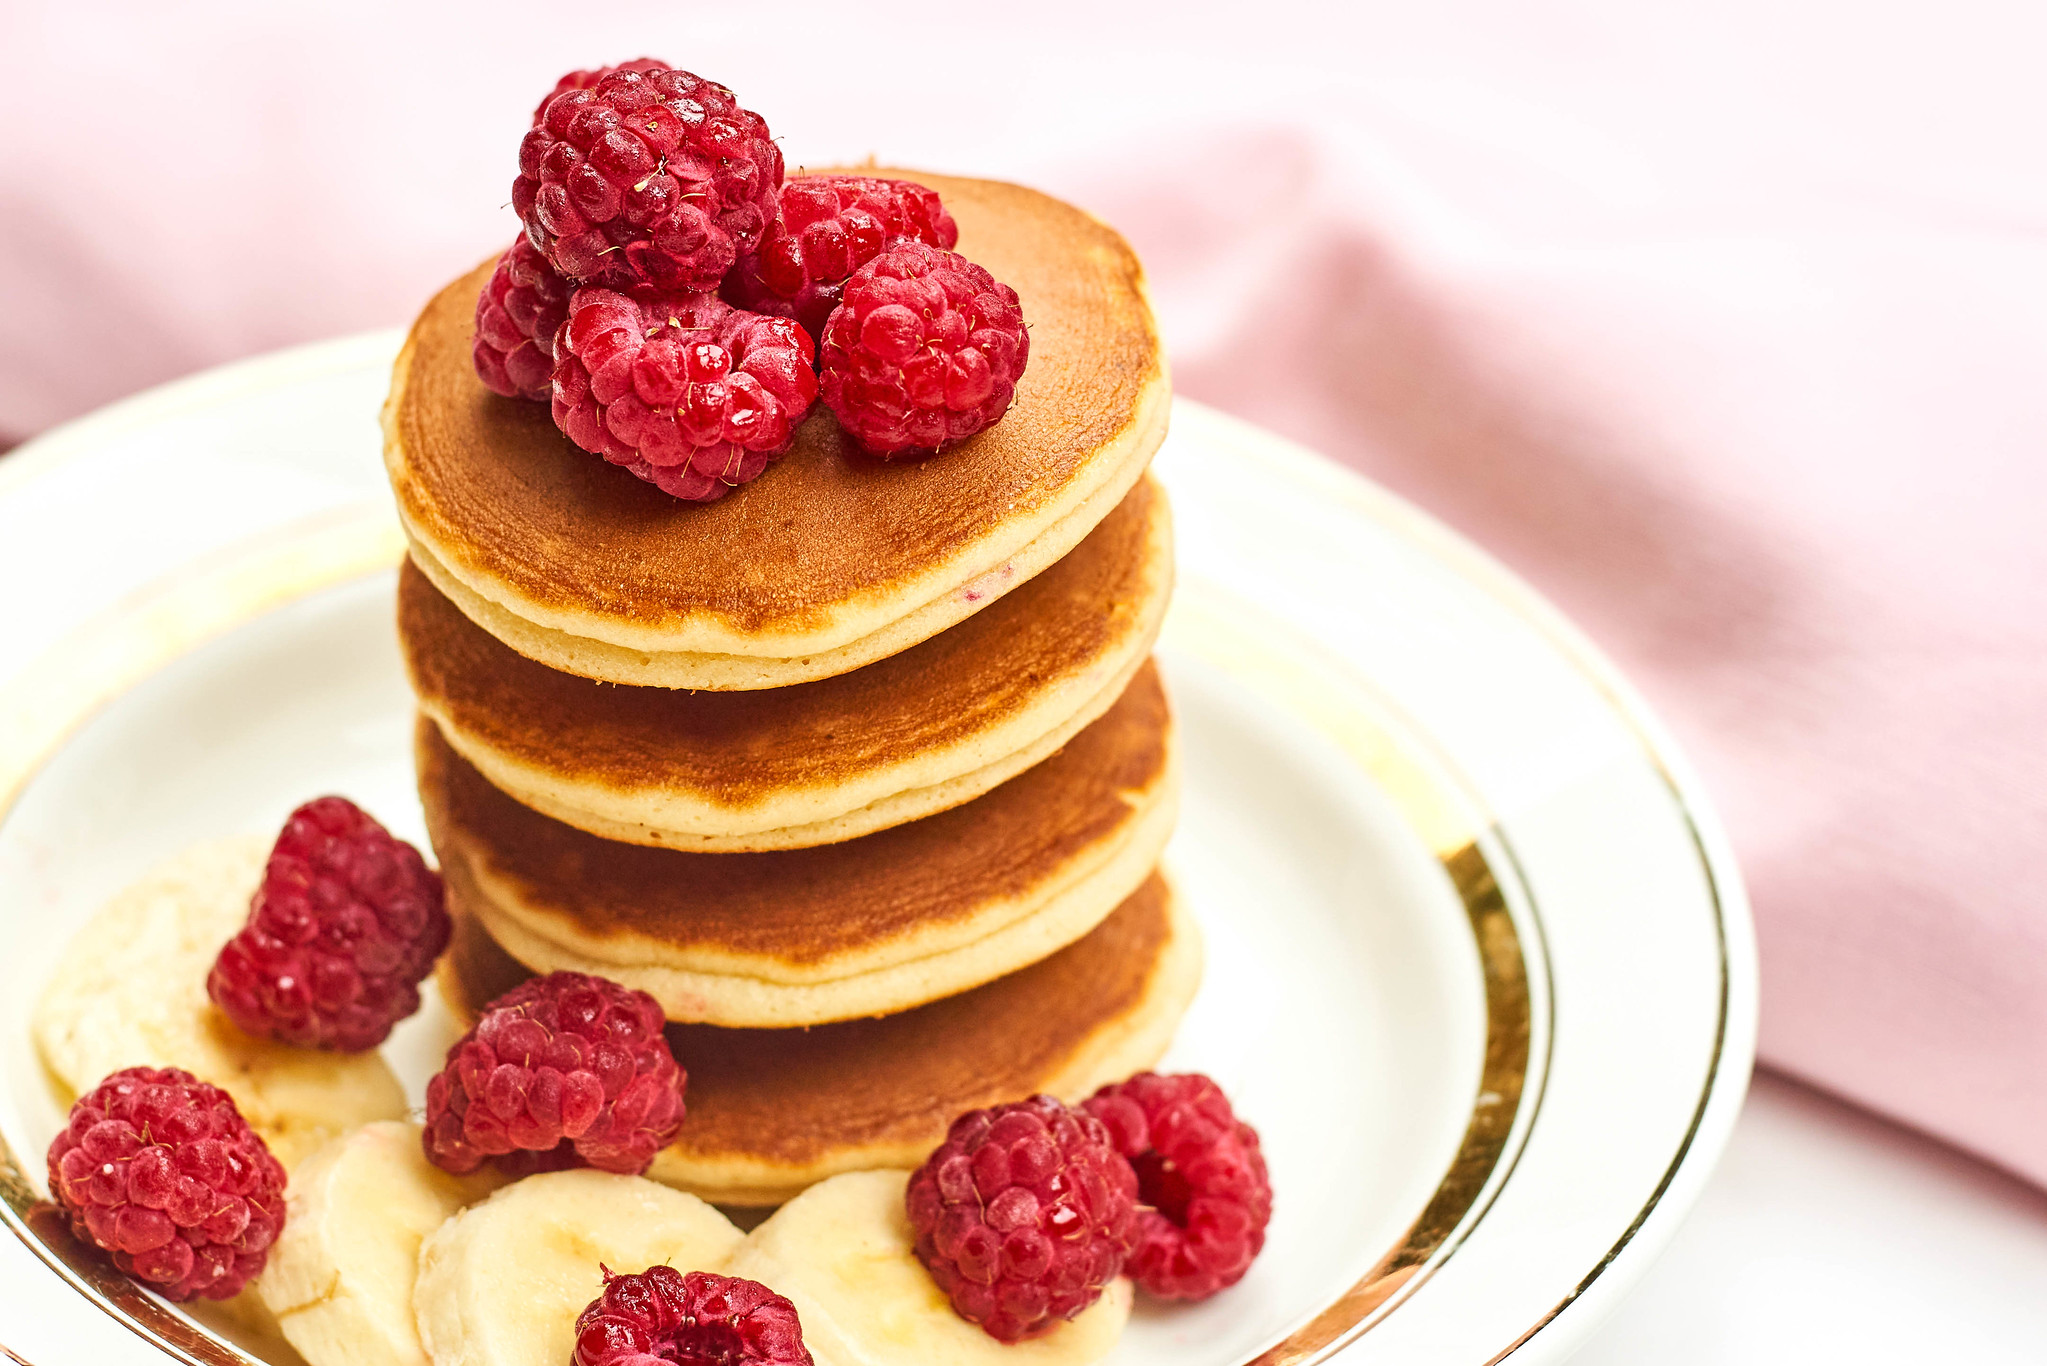
\includegraphics[width=180mm]{pancakes.jpg}
    \end{textblock*}
    \flattitle{150mm - \titlewidth}{5mm}{Stack-based languages}
\end{frame}

\begin{frame}[fragile]
    \frametitle{Pythagoras}
    \begin{onlyenv}<1- >%
    \rule[-30mm]{0pt}{60mm}%
    \begin{minipage}{80mm}%
        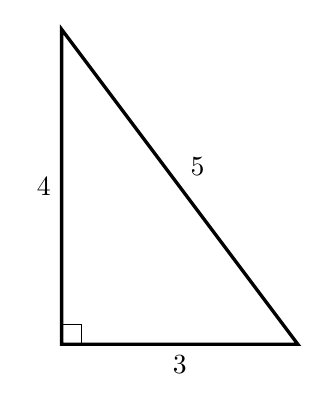
\begin{tikzpicture}[baseline={(current bounding box.center)}]
            \draw[very thick]
              (0,0) -- node[left] {4}
              (0,4) -- node[above right] {5}
              (3,0) -- node[below] {3} cycle;
            \draw[thin] (0,0.25) -- (0.25,0.25) -- (0.25,0);
        \end{tikzpicture}
    \end{minipage}%
    \end{onlyenv}%
    \begin{onlyenv}<2>%
    \rule[-30mm]{0pt}{60mm}%
    \begin{minipage}{45mm}%
        \begin{lstlisting}[language=python,gobble=8]
        import math
        print(math.sqrt(3*3 + 4*4))
        \end{lstlisting}
    \end{minipage}%
    \end{onlyenv}%
    \begin{onlyenv}<3>%
    \rule[-30mm]{0pt}{60mm}%
    \begin{minipage}{45mm}%
        \begin{lstlisting}[language=python,gobble=8]
        import math

        def pythogoras(leg1, leg2):
            l1sq = leg1 * leg1
            l2sq = leg2 * leg2
            hypotsq = l1sq + l2sq
            return math.sqrt(hypotsq)

        print(pythagoras(3, 4))
        print(pythagoras(5, 12))
        \end{lstlisting}
    \end{minipage}%
    \end{onlyenv}%
\end{frame}

\begin{frame}
    \frametitle{Programs operate on a stack}
    \stackex<+>{       }{ 1 2 + }
    \stackex<+>{      1}{ 2 + }
    \stackex<+>{    1 2}{ + }
    \stackex<+>{      3}{ }
\end{frame}

\begin{frame}
    \frametitle{The stack doesn't have to start empty}
    \stackex<+>{    1337 42}{ 1 2 + }
    \stackex<+>{  1337 42 1}{ 2 + }
    \stackex<+>{1337 42 1 2}{ + }
    \stackex<+>{  1337 42 3}{ }
\end{frame}

\begin{frame}
    \frametitle{Stack underflow is not fatal}
    \stackex<+>{         }{ 2 + }
    \stackex<+>{        2}{ + }
    \stackex<+>{2 \sym{+}}{ }
\end{frame}

\begin{frame}
    \frametitle{Pythagoras}
    \stackex<+>{       }{ 1 2 + 3 * 2 2 + 7 3 - * + sqrt }
    \stackex<+>{      1}{ 2 + 3 * 2 2 + 7 3 - * + sqrt }
    \stackex<+>{    1 2}{ + 3 * 2 2 + 7 3 - * + sqrt }
    \stackex<+>{      3}{ 3 * 2 2 + 7 3 - * + sqrt }
    \stackex<+>{    3 3}{ * 2 2 + 7 3 - * + sqrt }
    \stackex<+>{      9}{ 2 2 + 7 3 - * + sqrt }
    \stackex<+>{    9 2}{ 2 + 7 3 - * + sqrt }
    \stackex<+>{  9 2 2}{ + 7 3 - * + sqrt }
    \stackex<+>{    9 4}{ 7 3 - * + sqrt }
    \stackex<+>{  9 4 7}{ 3 - * + sqrt }
    \stackex<+>{9 4 7 3}{ - * + sqrt }
    \stackex<+>{  9 4 4}{ * + sqrt }
    \stackex<+>{   9 16}{ + sqrt }
    \stackex<+>{     25}{ sqrt }
    \stackex<+>{      5}{ }
\end{frame}

%%%%%%%%%%%%%%%%%%%%%%%%%%%%%%%%%%%%%%%%%%%%%%%%%%%%%%%%%%%%%%%%%%%%%%%%%%%%%%%%
% Concatenation and composition

\begin{frame}
    \begin{onlyenv}<+>
    \begin{center}
        \stacksplit[opacityback=0]{1 2 + 3 * 2}
        \stacksplit[opacityback=0]{2 + 7 3 - *}
        \stacksplit[opacityback=0]{+ sqrt}
    \end{center}
    \end{onlyenv}

    \begin{onlyenv}<+>
    \begin{center}
        \stacksplit[colback=red!20]{1 2 + 3 * 2}
        \stacksplit[colback=gray!20]{2 + 7 3 - *}
        \stacksplit[colback=yellow!20]{+ sqrt}
    \end{center}
    \end{onlyenv}
\end{frame}

%%%%%%%%%%%%%%%%%%%%%%%%%%%%%%%%%%%%%%%%%%%%%%%%%%%%%%%%%%%%%%%%%%%%%%%%%%%%%%%%

\begin{frame}[t]
    \frametitle{Picture credits}
    \begin{tabular}{lp{0.75\textwidth}}
    \picturecredits
    \end{tabular}
\end{frame}


\end{document}
